\documentclass{report}\usepackage[]{graphicx}\usepackage[]{color}
% maxwidth is the original width if it is less than linewidth
% otherwise use linewidth (to make sure the graphics do not exceed the margin)
\makeatletter
\def\maxwidth{ %
  \ifdim\Gin@nat@width>\linewidth
    \linewidth
  \else
    \Gin@nat@width
  \fi
}
\makeatother

\definecolor{fgcolor}{rgb}{0.345, 0.345, 0.345}
\makeatletter
\@ifundefined{AddToHook}{}{\AddToHook{package/xcolor/after}{\definecolor{fgcolor}{rgb}{0.345, 0.345, 0.345}}}
\makeatother
\newcommand{\hlnum}[1]{\textcolor[rgb]{0.686,0.059,0.569}{#1}}%
\newcommand{\hlstr}[1]{\textcolor[rgb]{0.192,0.494,0.8}{#1}}%
\newcommand{\hlcom}[1]{\textcolor[rgb]{0.678,0.584,0.686}{\textit{#1}}}%
\newcommand{\hlopt}[1]{\textcolor[rgb]{0,0,0}{#1}}%
\newcommand{\hlstd}[1]{\textcolor[rgb]{0.345,0.345,0.345}{#1}}%
\newcommand{\hlkwa}[1]{\textcolor[rgb]{0.161,0.373,0.58}{\textbf{#1}}}%
\newcommand{\hlkwb}[1]{\textcolor[rgb]{0.69,0.353,0.396}{#1}}%
\newcommand{\hlkwc}[1]{\textcolor[rgb]{0.333,0.667,0.333}{#1}}%
\newcommand{\hlkwd}[1]{\textcolor[rgb]{0.737,0.353,0.396}{\textbf{#1}}}%
\let\hlipl\hlkwb

\usepackage{framed}
\makeatletter
\newenvironment{kframe}{%
 \def\at@end@of@kframe{}%
 \ifinner\ifhmode%
  \def\at@end@of@kframe{\end{minipage}}%
  \begin{minipage}{\columnwidth}%
 \fi\fi%
 \def\FrameCommand##1{\hskip\@totalleftmargin \hskip-\fboxsep
 \colorbox{shadecolor}{##1}\hskip-\fboxsep
     % There is no \\@totalrightmargin, so:
     \hskip-\linewidth \hskip-\@totalleftmargin \hskip\columnwidth}%
 \MakeFramed {\advance\hsize-\width
   \@totalleftmargin\z@ \linewidth\hsize
   \@setminipage}}%
 {\par\unskip\endMakeFramed%
 \at@end@of@kframe}
\makeatother

\definecolor{shadecolor}{rgb}{.97, .97, .97}
\definecolor{messagecolor}{rgb}{0, 0, 0}
\definecolor{warningcolor}{rgb}{1, 0, 1}
\definecolor{errorcolor}{rgb}{1, 0, 0}
\makeatletter
\@ifundefined{AddToHook}{}{\AddToHook{package/xcolor/after}{
\definecolor{shadecolor}{rgb}{.97, .97, .97}
\definecolor{messagecolor}{rgb}{0, 0, 0}
\definecolor{warningcolor}{rgb}{1, 0, 1}
\definecolor{errorcolor}{rgb}{1, 0, 0}
}}
\makeatother
\newenvironment{knitrout}{}{} % an empty environment to be redefined in TeX

\usepackage{alltt}

\usepackage[usenames,dvipsnames,svgnames,table]{xcolor}

\usepackage[colorlinks=true,linkcolor=SteelBlue]{hyperref}

% set margins
\usepackage[margin=1in, headheight=3pt]{geometry}
%\geometry{left = 1in, right = 1in, top = 1in, bottom = 1in}

% set sof table figure
\usepackage{graphicx}
\usepackage{booktabs}
\usepackage{tabularx}
% \usepackage[T1]{fontenc}

\newcommand\soffignew[5]{

  \begin{table}
  \caption[SoF: #5]{Summary of findings: #5.}
             \label{tab:#1}
                 \begin{tabular}[width = \textwidth]{cc}
                 \hline
                 \includegraphics[width=0.4\textwidth]{#2} &
                                \includegraphics[width=0.5\textwidth]
                                {#3}\\
                   \hline
                   % sof
                   \multicolumn{2}{c}{
                     \includegraphics[width=0.95\textwidth]
                     {#4}
                   }\\
                   \hline
                   \end{tabular}
                   \end{table}
                 }

\newcommand\soffig[4]{

\begin{table}
\caption[SOF: #1]{Summary of findings: #4.}
\label{tab:#1}
\begin{tabular}[width = \textwidth]{cc}
pico here &

%
\includegraphics[width=0.5\textwidth]{#2} \\
% pico here & \includegraphics[width=0.5\textwidth]{img/#1- - -post_int-net.png}\\
\hline
% sof
\multicolumn{2}{c}{
\includegraphics[width=0.95\textwidth]{#3}
}\\
\hline
\end{tabular}
\end{table}

}












% set up frontmatter

\title{Supplementary material}
\IfFileExists{upquote.sty}{\usepackage{upquote}}{}
\begin{document}

\maketitle

\section{Table of contents}

\tableofcontents

\listoftables

\listoffigures


\chapter{Details about analyses}

\begin{itemize}

\item Funnel plots are shaded to show 90, 95, and 99 significance regions.

\end{itemize}

\chapter{Risk of bias summaries}

Figure \ref{fig:rob-grid} shows each study's risk of bias criteria and Figure \ref{fig:rob-bar} shows the distribution of risk of bias for each of the criteria.

\begin{figure}
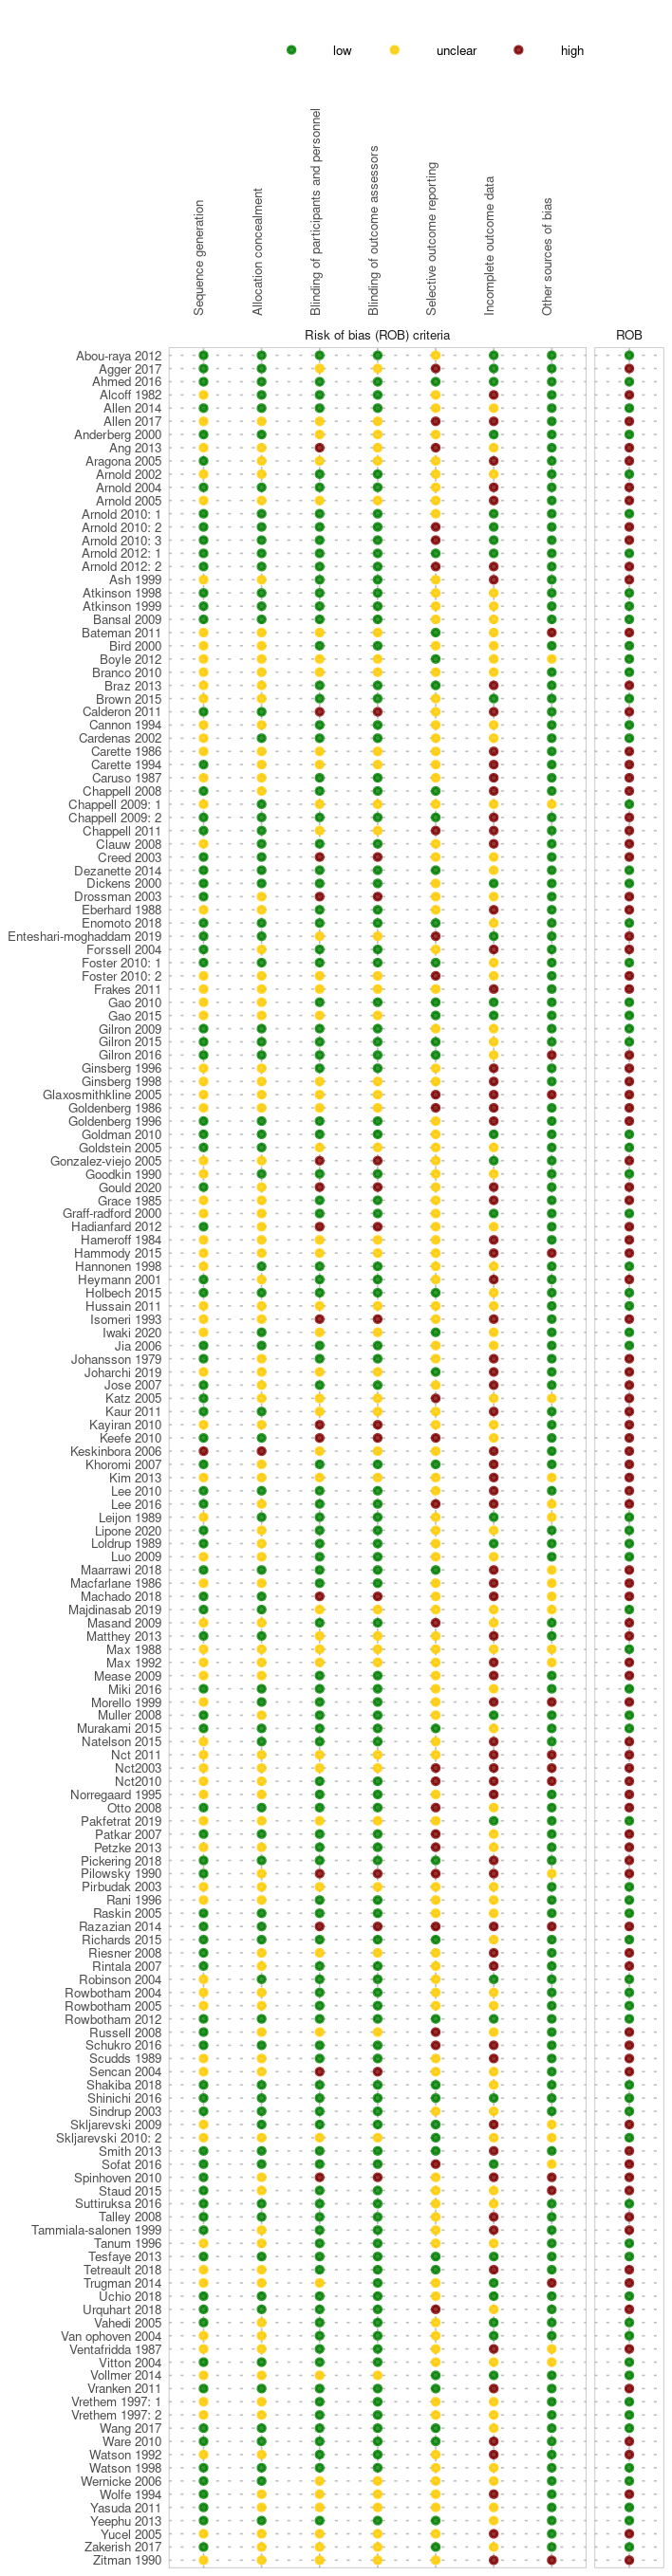
\includegraphics{img/rob-grid.png}
\caption{Risk of bias criteria for studies.}
\label{fig:rob-grid}
\end{figure}


\begin{figure}
\centering
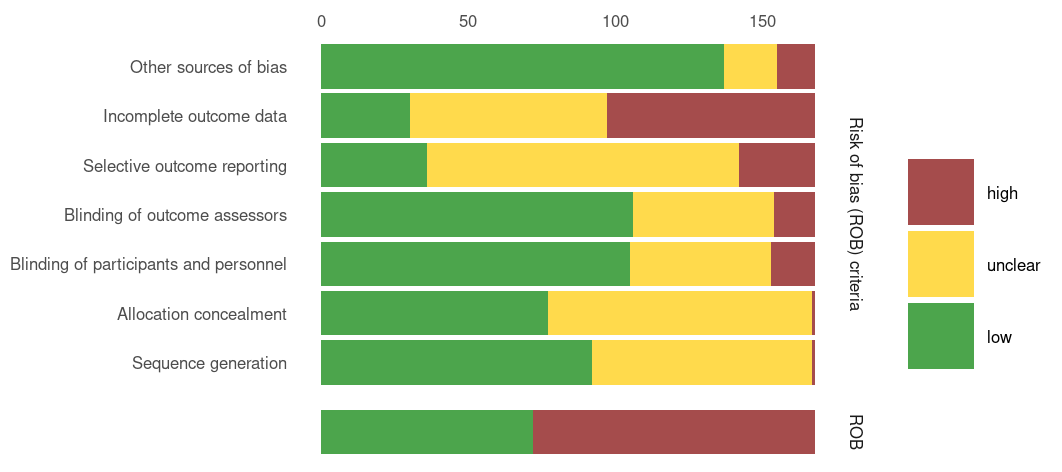
\includegraphics{img/rob-bar.png}
\caption{Risk of bias distributions for criteria.}
\label{fig:rob-bar}
\end{figure}


\chapter{Primary outcomes}

\section{Substantial pain relief}

Substantial pain relief was reported in 43 studies (5 crossover,  38 parallel design) including 14,880 participants and comparing 18 interventions for adults with chronic pain.  The length of trials ranged from 4 to 28 weeks, with the majority lasting 12 weeks. 7 studies did not include a placebo trial, comparing antidepressants with pregabalin (3 studies), gabapentin (1 study), morphine (1 study), and one study comparing amitriptyline with duloxetine without a placebo.

Interventions (18): placebo (36 studies); duloxetine (26); milnacipran (4); pregabalin (4); venlafaxine (3); desvenlafaxine (2); esreboxetine (2); mianserin (2); nortriptyline (2); amitriptyline (1); carbamazepine (1); clomipramine (1); gabapentin (1); imipramine (1); mirtazapine (1); morphine (1); nortriptyline + morphine (1); pregabalin + imipramine (1); trazodone + gabapentin (1).

Conditions (5):  neuropathic (19 studies); fibromyalgia (13); musculoskeletal (9); gastrointestinal (1); primary (1).

Summary of findings \ref{tab:painsub} shows the evidence network of post-intervention comparisons of treatments for chronic pain in adults. Of the 43 studies included, 36 had a placebo-controlled trial.

\soffignew
{painsub}
{img/pain_sub-post_int-net.png}
{img/pain_sub-pico.png}
{img/pain_sub-sof.png}
{Substantial pain relief (50\% reduction)}

\textbf{Duloxetine}: The NMA-estimated odds-ratio (OR) was 2.02 (95\% CI 1.72 to 2.37) for duloxetine, consistent with direct results. Majority of participants were fibromyalgia and neuropathic pain patients, in which subgroups the results were consistent. Duloxetine did not show these results at low doses, but was consistent across standard to high doses. Funnel plot asymmetry (Figure \ref{fig:painsub-dulox-plac}) suggests publication bias may be present.


Milnacipran: The NMA estimate (OR) was 1.67 (95\% CI 1.11 to 2.52) for milnacipran; these studies are primarily in fibromyalgia patients.

 The evidence for substantial pain relief is not consistent across interventions, and is focussed on SNRI-class antidepressant interventions. Thus, the results for other interventions are based on small evidence bases (low number of participants and or few studies).

The network meta-anlaysis results show significant substantial pain relief in chronic pain patients for SNRI antidepressants compared with placebo, with odds-ratios (OR) of between and 1 and 2.5 for duloxetine and milnacipran .

Appendix 2 provides meta-analyses, where the direct evidence is consistent with the results of the network meta-analysis. There was little inconsistency between results for fibromyalgia and neuropathic subgroups.  In terms of dose, there was only sufficient data for duloxetine, which only showed efficacy for standard and high doses,  whereas meta-analysis suggests duloxetine is ineffective at low doses.

\subsection{Head to head comparisons and subgroup sensitivity analyses}


Duloxetine did not show inconsistency or imprecision, within the meta-analysis, and compared to the network meta-analysis estimates, however some funnel plot asymmetry suggests publication bias (Figure \ref{fig:painsub-dulox-plac}).

\subsubsection{Duloxetine}

\begin{figure}

\begin{knitrout}
\definecolor{shadecolor}{rgb}{0.969, 0.969, 0.969}\color{fgcolor}
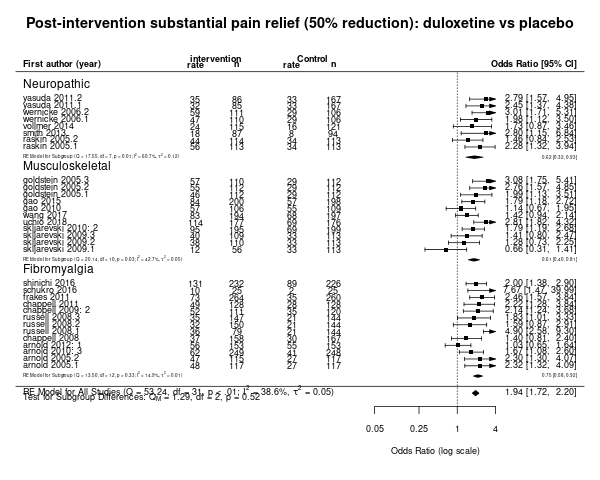
\includegraphics[width=0.5\linewidth,height=0.35\textheight]{img/pain_sub-duloxetine-placebo-forest} 
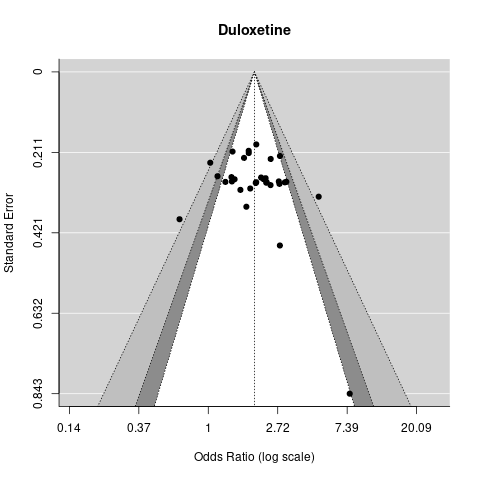
\includegraphics[width=0.5\linewidth,height=0.35\textheight]{img/pain_sub-duloxetine-placebo-funnel} 
\end{knitrout}

\caption{
%\include{"pain\_sub-duloxetine-placebo-rma-caption.txt"}
}
\label{fig:painsub-dulox-plac}
\end{figure}


\subsubsection{Milnacipran}

Meta-analysis of milnacipran was consistent with network meta-analysis estimates. No inconsistency, imprecision, or publication bias detected, however, one third of studies included were high risk of bias.


Duloxetine (Figure \ref{fig:painsub-dulox-plac}), milnacipran (Figure \ref{fig:subpain-milna}), and esreboxetine (Figure \ref{fig:subpain-esrebox}) all show significant substantial pain relief (measured as 50 per cent reduction at post-intervention) compared with placebo. Duloxetine trials show some funnel plot asymmetry; more serious asymmetry was detected for milnacipran.


There were not enough trials for a meaningful meta-analysis of milnacipran, amitriptyline, and esreboxetine for most subgroup analyses. Esreboxetine and milnacipran results were primarily in fibromyalgia patients. We found sufficient trials to consider whether various subgroups account for variation in duloxetine results.

Conditions: Duloxetine shows significant improvement for neuropathic pain patients (Figure \ref{fig:subpain-neuro-dulox}), and those with fibromyalgia (Figure \ref{fig:subpain-fibro-dulox}); asymmetry was not significant. Milnacipran also showed significant improvement for fibromyalgia (Figure \ref{fig:subpain-fibro-milna}).

\begin{figure}

\begin{knitrout}
\definecolor{shadecolor}{rgb}{0.969, 0.969, 0.969}\color{fgcolor}
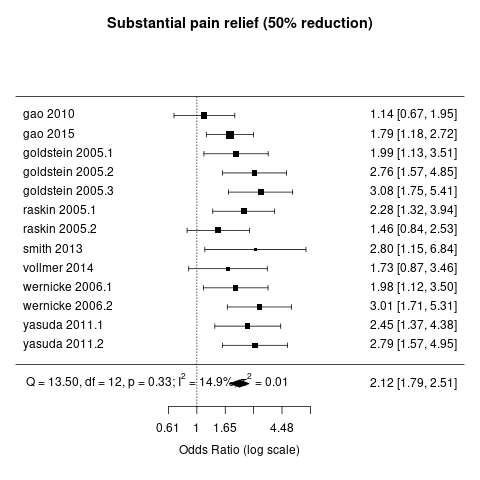
\includegraphics[width=0.5\linewidth,height=0.35\textheight]{img/pain_sub-duloxetine-condition-neuropathic-forest} 
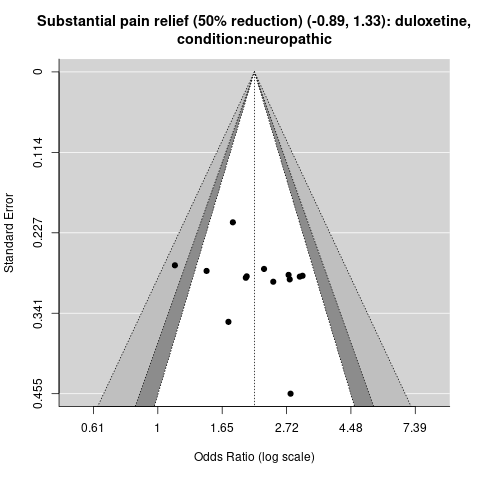
\includegraphics[width=0.5\linewidth,height=0.35\textheight]{img/pain_sub-duloxetine-condition-neuropathic-funnel} 
\end{knitrout}

\caption[Substantial pain: duloxetine, neuropathic]{Outcome: Substantial pain relief  (50 per cent reduction). Measure: post-intervention. Intervention: duloxetine. Condition: neuropathic. Participants: 3091. Meta-analysis results: Q = 13.5; df = 12; p = 0.33; $I^2$ = 14.95 per cent; $\tau^2$ = 0.01. Regression test for funnel plot asymmetry was not significant: 0.22 (CI -0.89 to 1.33) with p = 0.34 and z = 0.95.}
\label{fig:subpain-neuro-dulox}
\end{figure}

There were not enough trials for a meaningful meta-analysis of milnacipran, amitriptyline, and esreboxetine for most subgroup analyses. Esreboxetine and milnacipran results were primarily in fibromyalgia patients. We found sufficient trials to consider whether various subgroups account for variation in duloxetine results.


\begin{figure}

\begin{knitrout}
\definecolor{shadecolor}{rgb}{0.969, 0.969, 0.969}\color{fgcolor}
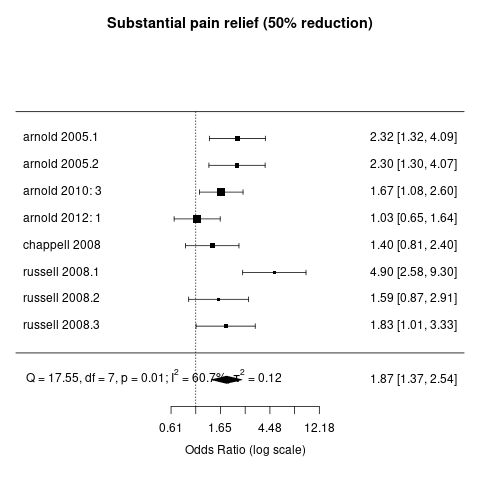
\includegraphics[width=0.5\linewidth,height=0.35\textheight]{img/pain_sub-duloxetine-condition-fibromyalgia-forest} 
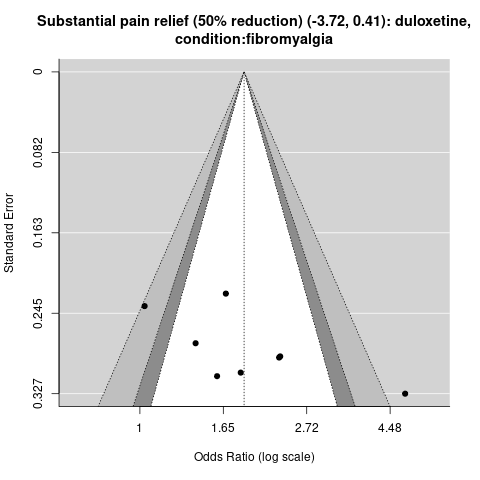
\includegraphics[width=0.5\linewidth,height=0.35\textheight]{img/pain_sub-duloxetine-condition-fibromyalgia-funnel} 
\end{knitrout}

\caption[Substantial pain: duloxetine, fibromyalgia]{Outcome: Substantial pain relief  (50 per cent reduction). Measure: post-intervention. Intervention: duloxetine. Condition: fibromyalgia. Participants: 2402. Meta-analysis results: Q = 17.55; df = 7; p = 0.01; $I^2$ = 60.68 per cent; $\tau^2$ = 0.12. Regression test for funnel plot asymmetry was not significant: -1.65 (CI -3.72 to 0.41) with p = 0.03 and z = 2.17.
}
\label{fig:subpain-fibro-dulox}
\end{figure}

\begin{figure}

\begin{knitrout}
\definecolor{shadecolor}{rgb}{0.969, 0.969, 0.969}\color{fgcolor}
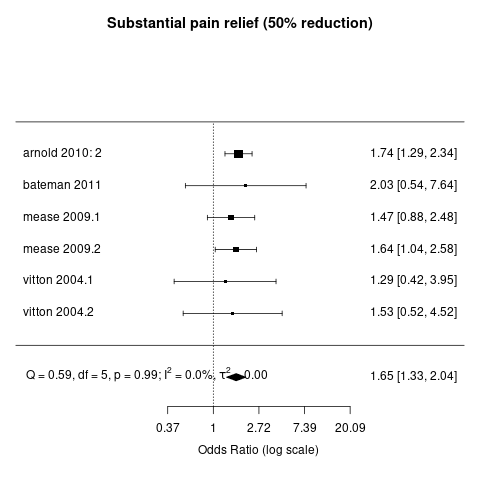
\includegraphics[width=0.5\linewidth,height=0.35\textheight]{img/pain_sub-milnacipran-condition-fibromyalgia-forest} 
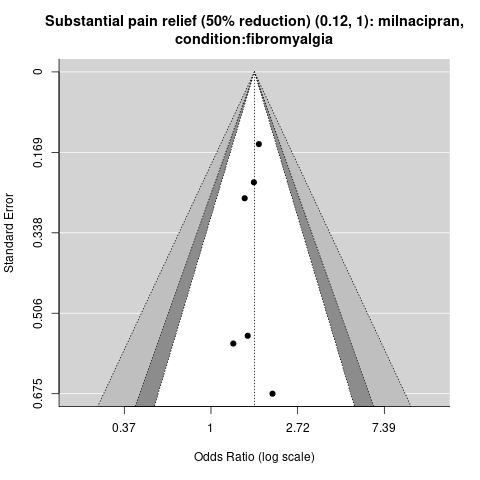
\includegraphics[width=0.5\linewidth,height=0.35\textheight]{img/pain_sub-milnacipran-condition-fibromyalgia-funnel} 
\end{knitrout}

\caption[Substantial pain: milnacipran, fibromyalgia]{Outcome: Substantial pain relief  (50 per cent reduction). Measure: post-intervention. Intervention: milnacipran. Condition: fibromyalgia. Participants: 1935. Meta-analysis results: Q = 0.59; df = 5; p = 0.99; $I^2$ = 0 per cent; $\tau^2$ = 0. Regression test for funnel plot asymmetry was significant: 0.56 (CI 0.12 to 1) with p = 0.76 and z = -0.31.
}
\label{fig:subpain-fibro-milna}
\end{figure}

Dose: Evidence supports duloxetine at high (Figure \ref{fig:subpain-highdose-dulox}) and standard (Figure \ref{fig:subpain-standarddose-dulox}) doses, but not at low (Figure \ref{fig:subpain-lowdose-dulox}).

\begin{figure}

\begin{knitrout}
\definecolor{shadecolor}{rgb}{0.969, 0.969, 0.969}\color{fgcolor}
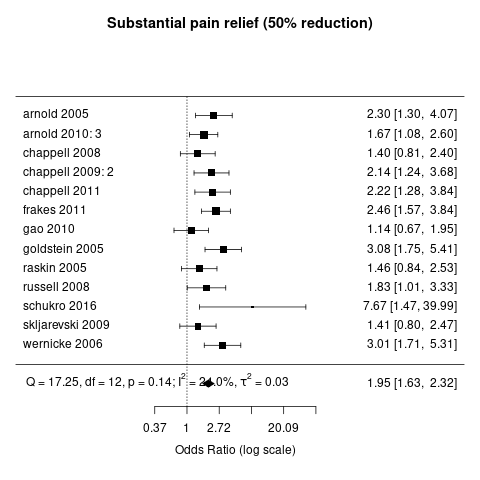
\includegraphics[width=0.5\linewidth,height=0.35\textheight]{img/pain_sub-duloxetine-dose-high-forest} 
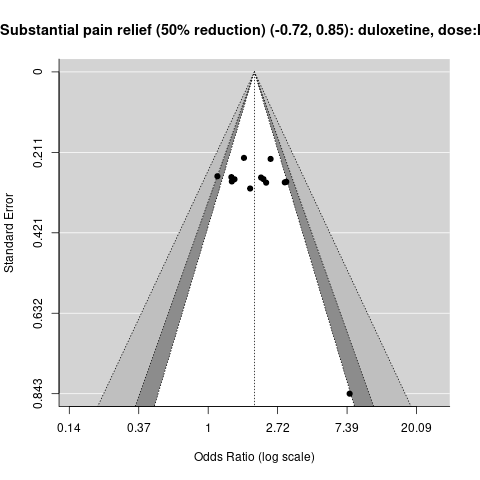
\includegraphics[width=0.5\linewidth,height=0.35\textheight]{img/pain_sub-duloxetine-dose-high-funnel} 
\end{knitrout}

\caption[Substantial pain: duloxetine, high dose]{Outcome: Substantial pain relief  (50 per cent reduction). Measure: post-intervention. Intervention: duloxetine. Dose: high. Participants: 3509. Meta-analysis results: Q = 17.25; df = 12; p = 0.14; $I^2$ = 24.03 per cent; $\tau^2$ = 0.03. Regression test for funnel plot asymmetry was not significant: 0.07 (CI -0.72 to 0.85) with p = 0.13 and z = 1.53.
}
\label{fig:subpain-highdose-dulox}
\end{figure}

\begin{figure}

\begin{knitrout}
\definecolor{shadecolor}{rgb}{0.969, 0.969, 0.969}\color{fgcolor}
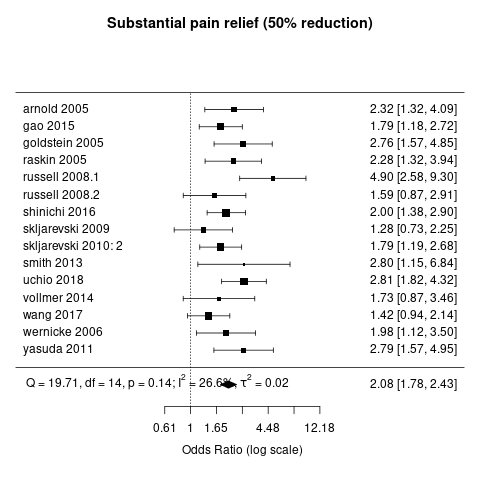
\includegraphics[width=0.5\linewidth,height=0.35\textheight]{img/pain_sub-duloxetine-dose-standard-forest} 
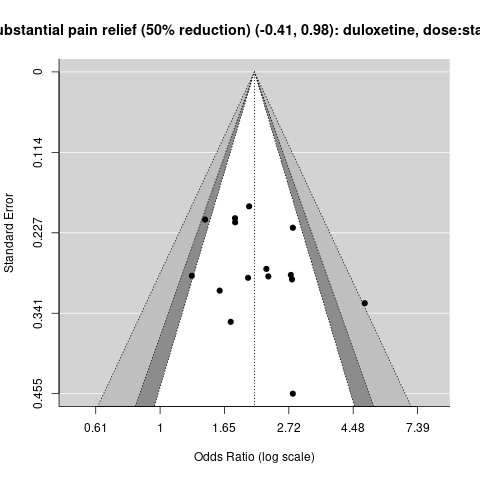
\includegraphics[width=0.5\linewidth,height=0.35\textheight]{img/pain_sub-duloxetine-dose-standard-funnel} 
\end{knitrout}

\caption[Substantial pain: duloxetine, standard dose]{Outcome: Substantial pain relief  (50 per cent reduction). Measure: post-intervention. Intervention: duloxetine. Dose: standard. Participants: 4304. Meta-analysis results: Q = 19.71; df = 14; p = 0.14; $I^2$ = 26.63 per cent; $\tau^2$ = 0.02. Regression test for funnel plot asymmetry was not significant: 0.28 (CI -0.41 to 0.98) with p = 0.2 and z = 1.29.
}
\label{fig:subpain-standarddose-dulox}
\end{figure}

\begin{figure}

\begin{knitrout}
\definecolor{shadecolor}{rgb}{0.969, 0.969, 0.969}\color{fgcolor}
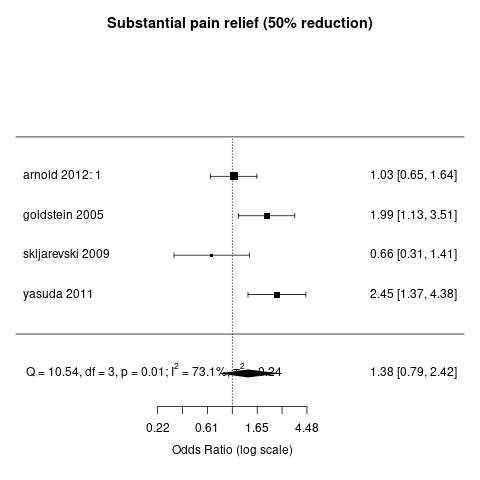
\includegraphics[width=0.5\linewidth,height=0.35\textheight]{img/pain_sub-duloxetine-dose-low-forest} 
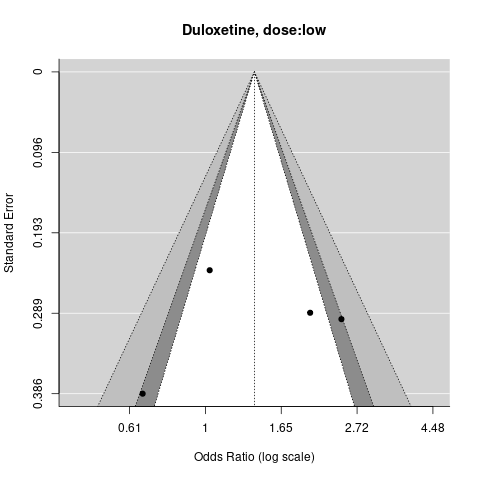
\includegraphics[width=0.5\linewidth,height=0.35\textheight]{img/pain_sub-duloxetine-dose-low-funnel} 
\end{knitrout}

\caption[Substantial pain: duloxetine, low dose]{Outcome: Substantial pain relief  (50 per cent reduction). Measure: post-intervention. Intervention: duloxetine. Dose: low. Participants: 951. Meta-analysis results: Q = 10.54; df = 3; p = 0.01; $I^2$ = 73.09 per cent; $\tau^2$ = 0.24. Regression test for funnel plot asymmetry was not significant: 1.48 (CI -2.3 to 5.26) with p = 0.54 and z = -0.61.
}
\label{fig:subpain-lowdose-dulox}
\end{figure}


Risk of bias: Subgroup analyses of risk of bias (Figure \ref{fig:subpain-highrob-dulox}) showed no difference in consistency and precision for duloxetine. Aside from an outlier for high risk of bias in duloxetine, the subgroups' funnel plots do not show significant asymmetry (Figure \ref{fig:subpain-lowrob-dulox}).

\begin{figure}

\begin{knitrout}
\definecolor{shadecolor}{rgb}{0.969, 0.969, 0.969}\color{fgcolor}
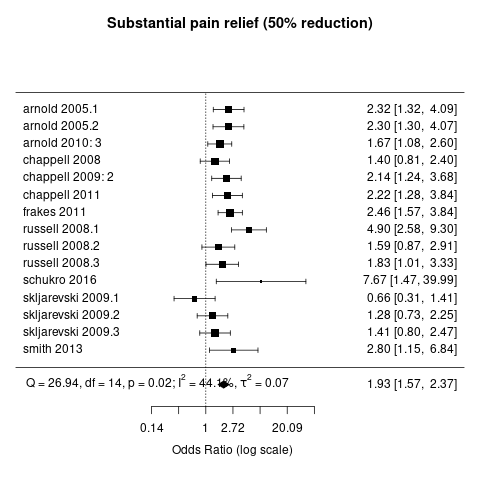
\includegraphics[width=0.5\linewidth,height=0.35\textheight]{img/pain_sub-duloxetine-rob-high-forest} 
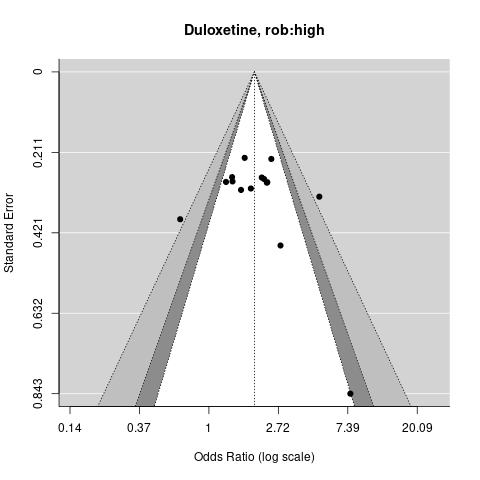
\includegraphics[width=0.5\linewidth,height=0.35\textheight]{img/pain_sub-duloxetine-rob-high-funnel} 
\end{knitrout}

\caption[Substantial pain: duloxetine, high ROB]{Outcome: Substantial pain relief  (50 per cent reduction). Measure: post-intervention. Intervention: duloxetine. ROB: high. Participants: 3952. Meta-analysis results: Q = 26.94; df = 14; p = 0.02; $I^2$ = 44.15 per cent; $\tau^2$ = 0.07. Regression test for funnel plot asymmetry was not significant: 0.21 (CI -0.59 to 1.01) with p = 0.26 and z = 1.14.
}
\label{fig:subpain-highrob-dulox}
\end{figure}

\begin{figure}

\begin{knitrout}
\definecolor{shadecolor}{rgb}{0.969, 0.969, 0.969}\color{fgcolor}
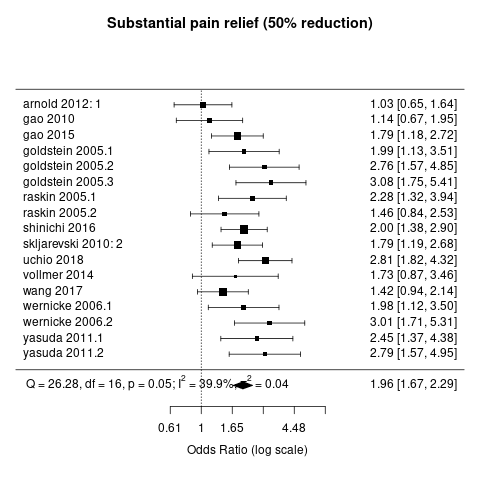
\includegraphics[width=0.5\linewidth,height=0.35\textheight]{img/pain_sub-duloxetine-rob-low-forest} 
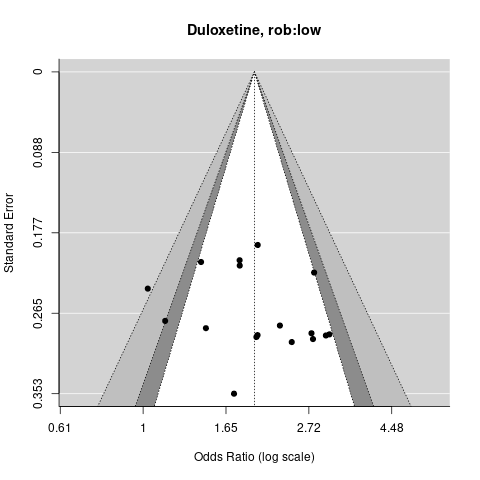
\includegraphics[width=0.5\linewidth,height=0.35\textheight]{img/pain_sub-duloxetine-rob-low-funnel} 
\end{knitrout}

\caption[Substantial pain: duloxetine, low ROB]{Outcome: Substantial pain relief  (50 per cent reduction). Measure: post-intervention. Intervention: duloxetine. ROB: low. Participants: 4812. Meta-analysis results: Q = 26.28; df = 16; p = 0.05; $I^2$ = 39.92 per cent; $\tau^2$ = 0.04. Regression test for funnel plot asymmetry was not significant: 0.18 (CI -0.78 to 1.14) with p = 0.31 and z = 1.02
}
\label{fig:subpain-lowrob-dulox}
\end{figure}

\newpage

\section{Pain intensity (continuous scales)}


\subsection{Change scores}

Pain intensity was reported in 46 studies (3 crossover, 43 parallel) evaluating 46 interventions in trials comprising 14,887 total participants. Studies ran from 5 to 52 weeks, with median length 12 weeks. In the trials reporting placebo, most compared interventions with placebo; with exceptions XX. The geometry of the network is ...



\soffignew
{painint}
{img/pain_int-change_score-net.png}
{img/pain_int-change_score-pico.png}
{img/pain_int-change_score-sof.png}
{Pain intensity (change score measures)}


\subsection{Post intervention}


Pain intensity was reported as a post-intervention measure in 80 studies (18 crossover, 62 parallel) evaluating 70 interventions in trials comprising a total of 8016 participants. Studies ran from 2 to 36 weeks, with median length 8 weeks.


\soffignew
{painint}
{img/pain_int-post_int-net.png}
{img/pain_int-post_int-pico.png}
{img/pain_int-post_int-sof.png}
{Pain intensity (post-intervention measures)}


\textbf{Interventions} (number of studies):

\section{Mood}

Mood was reported in 145 studies with 71 studies reporting change score (CS) measures (0 crossover, 98 parallel design) and 74 studies reporting post intervention (PI) measures (26 crossover, 96 parallel design). These trials include 16,808 participants (CS 13,004, PI 3804) and comparing 66 interventions (CS 17, PI 49) for adults with chronic pain. The length of trials ranged from 2 to 52 weeks, with the majority lasting 12 weeks. The direct evidence networks for the two measurement groups are shown in Summary of findings Tables \ref{tab:moodcs} and \ref{tab:moodpi}.

\subsection{Change score results}

Three studies did not include placebo trials, using cognitive behavioural therapy, pregabalin, and psychotherapy as comparators with antidepressants.

\soffignew
{moodcs}
{img/mood-change_score-net.png}
{img/mood-change_score-pico.png}
{img/mood-change_score-sof.png}
{Mood (change-score measures)}


\textbf{Interventions} (number of studies): Placebo (33); duloxetine (26); milnacipran (4); citalopram (2); pregabalin (2); abt-894 (1); cbt (1); cbt and milnacipran (1); desipramine (1); desipramine + lidocaine (1); esreboxetine (1); fluoxetine (1); imipramine (1); lidocaine (1); mirtazapine (1); nortriptyline (1); paroxetine (1); psychotherapy (1); usual treatment (1).

Conditions: fibromyalgia; musculoskeletal; neuropathic; gastrointestinal; vulvodynia.

Summary of findings (Table \ref{tab:moodcs}) shows 26 studies evaluated duloxetine, 4 studies evaluatede milnacipran, and all other interventions were evalatuated in 1 or 2 studies.



\subsection{Post intervention results}

For post-intervention measures, several other comparators were considered in the literature, notably amitriptyline (7 studies), citalopram (2 studies), fluoxetine (2 studies), and acupuncture (2 studies). Most comparators were either combined or unique, with trials included in only one study.

\soffignew
{moodpi}
{img/mood-post_int-net.png}
{img/mood-post_int-pico.png}
{img/mood-post_int-sof.png}
{Mood (post-intervention measures)}



\textbf{Interventions} (number of studies): Placebo (27); amitriptyline (10); duloxetine (8); benzotropine mesylate (4); fluoxetine (4); pregabalin (4); venlafaxine (4); escitalopram (3); milnacipran (3); nortriptyline (3); paroxetine (3); acupuncture (2); cbt (2); citalopram (2); morphine (2); saffron/crocin (2); aerobic exercise (1); amitriptyline + fluoxetine (1); amitriptyline + fluphenazine (1); amitriptyline + riboflavin (vitamin b2) (1); amitriptyline + splint (1); carbamazepine (1); clomipramine (1); cst (1); cst + sertraline (1); cyclobenzaprine (1); disease management (1); dothiepin (1); fluoxetine + melatonin (1); fluphenazine (1); gabapentin (1); gabapentin + nortriptyline (1); glycopyrrolate (1); maprotiline (1); melatonin (1); mirtazapine (1); moclobemide (1); morphine + nortriptyline (1); neurofeedback (1); nortriptyline + cbt (1); nortriptyline + disease management (1); nortriptyline + morphine (1); pirlindole (1); pregabalin + duloxetine (1); reboxetine (1); riboflavin (vitamin b2) (1); sertraline (1); tens (1); trazodone (1); trimipramine (1); waitlist (1).

Conditions: musculoskeletal; primary; neuropathic; fibromyalgia; atypical facial pain; non-cardiac chest pain; burning mouth syndrome; phantom/residual limb pain; unspecified.

In Summary of Findings Table \ref{tab:moodpi}, there are 10 studies that evaluate amitriptyline and 8 that evaluate duloxetine. Of the 50 interventions evaluated, most are included in 3 studies or fewer.

\subsubsection{meta-analyses analyses}

meta-analyses results for duloxetine in \ref{fig:mood-cs-dulox}

\begin{figure}

\begin{knitrout}
\definecolor{shadecolor}{rgb}{0.969, 0.969, 0.969}\color{fgcolor}
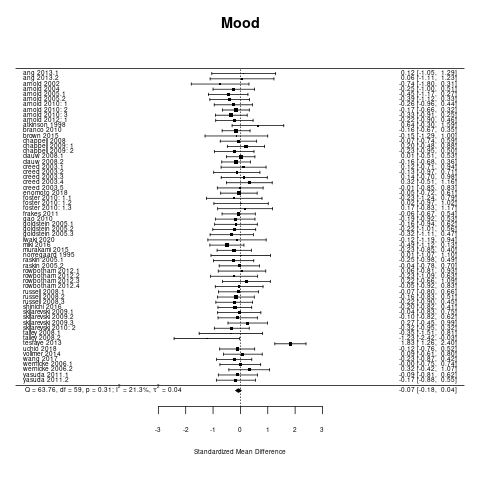
\includegraphics[width=0.5\linewidth,height=0.35\textheight]{img/mood-change_score-duloxetine- - -forest} 
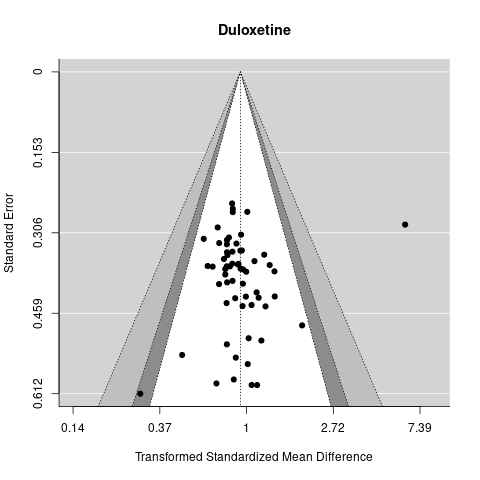
\includegraphics[width=0.5\linewidth,height=0.35\textheight]{img/mood-change_score-duloxetine- - -funnel} 
\end{knitrout}

\caption[Mood: duloxetine]{Outcome: mood. Measure: change score. Intervention: duloxetine. Participants: 951. Direction of improvement: lower. Meta-analysis results: Q = 10.54; df = 3; p = 0.01; $I^2$ = 73.09 per cent; $\tau^2$ = 0.24. Regression test for funnel plot asymmetry was not significant: 1.48 (CI -2.3 to 5.26) with p = 0.54 and z = -0.61.}
\label{fig:mood-cs-dulox}
\end{figure}


\section{Adverse events}


Adverse events were reported in 91 studies (15 crossover, 76 parallel design) including 22,025 participants and comparing 46 interventions for adults with chronic pain. The length of trials ranged from 2 to 52 weeks, with the majority lasting about 10 weeks.

\soffignew{adverse}{img/adverse- - -post_int-net.png}{img/adverse-pico.png}{img/adverse-sof.png}{Adverse events}


\subsection{Meta-analyses}

\subsubsection{Duloxetine}

The direct evidence for duloxetine compared with placebo was consistent with the network meta-analysis estimates, however publication bias (Figure \ref{fig:adverse-dulox-plac}) is strongly suspected, also implied by the comparison of duloxetine and pregabalin (Figure \ref{fig:adverse-dulox-pregab}).

\begin{figure}
\begin{knitrout}
\definecolor{shadecolor}{rgb}{0.969, 0.969, 0.969}\color{fgcolor}
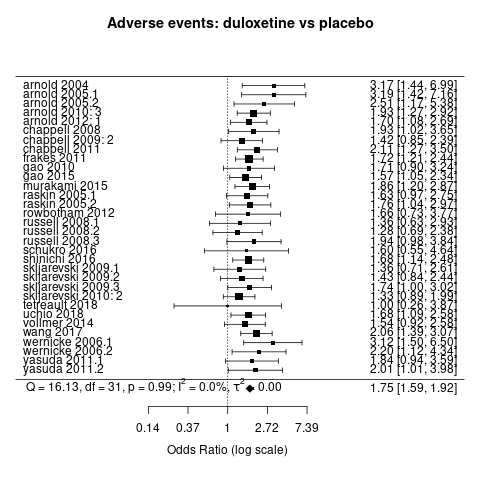
\includegraphics[width=0.5\linewidth,height=0.35\textheight]{img/adverse-duloxetine-placebo-forest} 
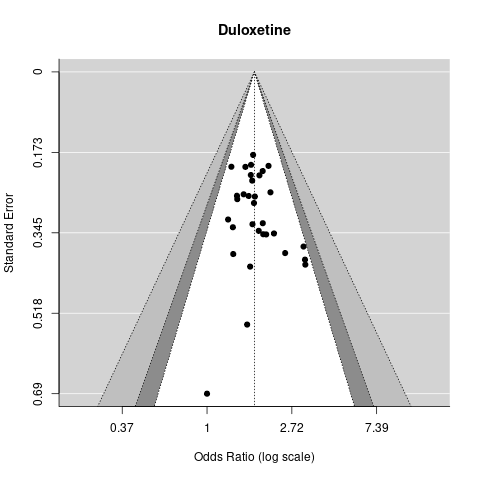
\includegraphics[width=0.5\linewidth,height=0.35\textheight]{img/adverse-duloxetine-placebo-funnel} 
\end{knitrout}

\caption[Adverse: duloxetine vs pregabalin]{\input{img/adverse-duloxetine-placebo-rma-caption.txt}}
\label{fig:adverse-dulox-plac}
\end{figure}




\begin{figure}
\begin{knitrout}
\definecolor{shadecolor}{rgb}{0.969, 0.969, 0.969}\color{fgcolor}
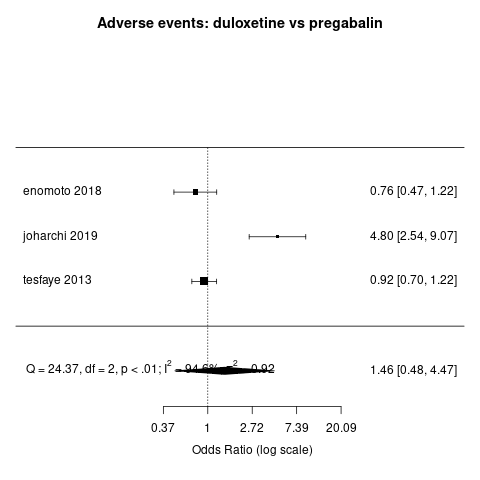
\includegraphics[width=0.5\linewidth,height=0.35\textheight]{img/adverse-duloxetine-pregabalin-forest} 
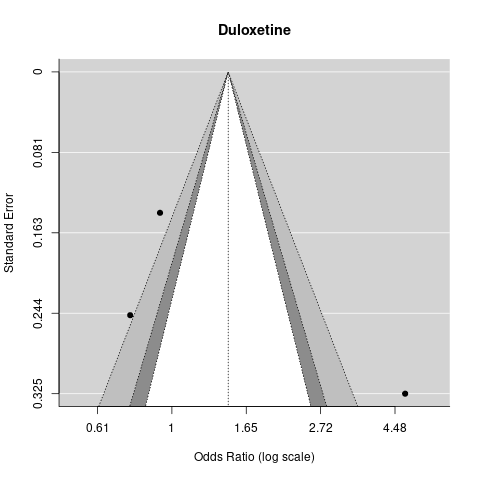
\includegraphics[width=0.5\linewidth,height=0.35\textheight]{img/adverse-duloxetine-pregabalin-funnel} 
\end{knitrout}

\caption[Adverse: duloxetine vs pregabalin]{\input{img/adverse-duloxetine-pregabalin-rma-caption.txt}}
\label{fig:adverse-dulox-pregab}
\end{figure}



\begin{figure}

\begin{knitrout}
\definecolor{shadecolor}{rgb}{0.969, 0.969, 0.969}\color{fgcolor}
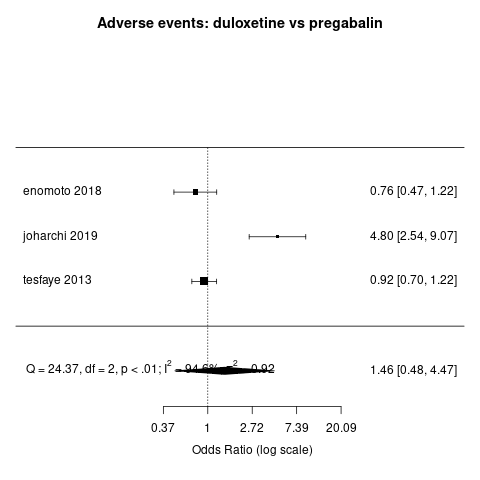
\includegraphics[width=0.5\linewidth,height=0.35\textheight]{img/adverse-duloxetine- - -forest} 
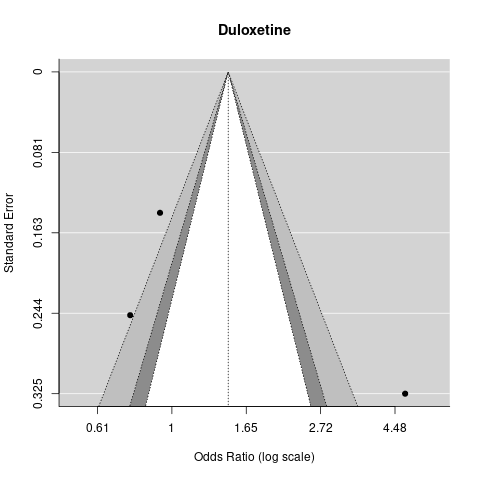
\includegraphics[width=0.5\linewidth,height=0.35\textheight]{img/adverse-duloxetine- - -funnel} 
\end{knitrout}

\caption[Adverse events: duloxetine]{Outcome: adverse events. Measure: post-intervention. Intervention: duloxetine. Participants: 8791. Direction of improvement: lower. Meta-analysis results: Q = 16.13; df = 31; p = 0.99; $I^2$ = 0 per cent; $\tau^2$ = 0. Regression test for funnel plot asymmetry was significant: 0.42 (CI 0.08 to 0.76) with p = 0.41 and z = 0.82.}
\label{fig:adverse-dulox}
\end{figure}

\begin{figure}

\begin{knitrout}
\definecolor{shadecolor}{rgb}{0.969, 0.969, 0.969}\color{fgcolor}
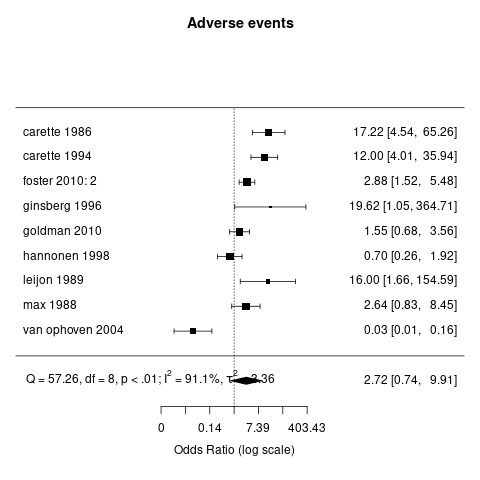
\includegraphics[width=0.5\linewidth,height=0.35\textheight]{img/adverse-amitriptyline- - -forest} 
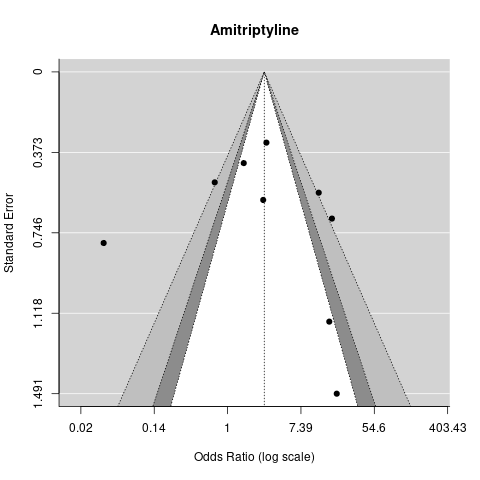
\includegraphics[width=0.5\linewidth,height=0.35\textheight]{img/adverse-amitriptyline- - -funnel} 
\end{knitrout}

\caption[Adverse events: amitriptyline]{Outcome: adverse events. Measure: post-intervention. Intervention: amitriptyline. Participants: 915. Direction of improvement: lower. Meta-analysis results: Q = 57.26; df = 8; p $<$ .01; $I^2$ = 91.1 per cent; $\tau^2$ = 3.36. Regression test for funnel plot asymmetry was not significant: -0.13 (CI -3.25 to 2.99) with p = 0.43 and z = 0.79.}
\label{fig:adverse-amitrip}
\end{figure}



\begin{figure}

\begin{knitrout}
\definecolor{shadecolor}{rgb}{0.969, 0.969, 0.969}\color{fgcolor}
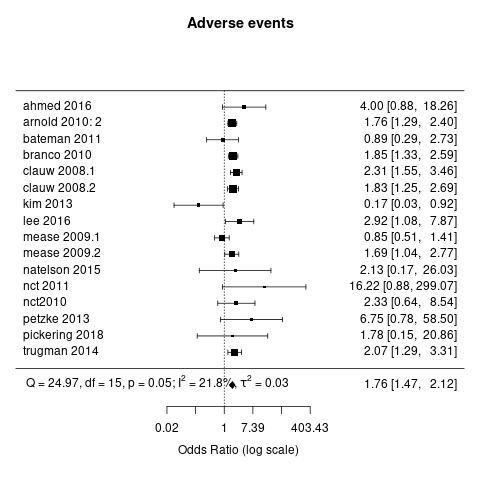
\includegraphics[width=0.5\linewidth,height=0.35\textheight]{img/adverse-milnacipran- - -forest} 
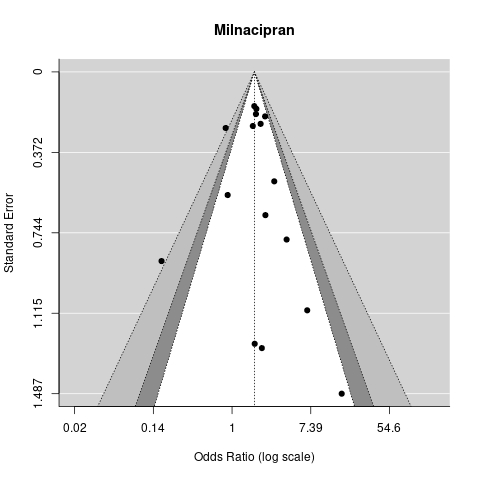
\includegraphics[width=0.5\linewidth,height=0.35\textheight]{img/adverse-milnacipran- - -funnel} 
\end{knitrout}

\caption[Adverse events: milnacipran]{Outcome: adverse events. Measure: post-intervention. Intervention: milnacipran. Participants: 5455. Direction of improvement: lower. Meta-analysis results: Q = 24.97; df = 15; p = 0.05; $I^2$ = 21.85 per cent; $\tau^2$ = 0.03. Regression test for funnel plot asymmetry was significant: 0.51 (CI 0.2 to 0.83) with p = 0.69 and z = 0.4.}
\label{fig:adverse-amitrip}
\end{figure}

\chapter{Secondary outcomes}


\section{Serious adverse events (SAE)}

SAE were reported in 60 studies (8 crossover, 52 parallel) evaluating 30 interventions including 16,138 participants with one of seven pain conditions. The studies ranged from  2 to 34 weeks with most studies lasting 12 weeks. Summary of findings \ref{tab:serious} shows the direct evidence network for SAE wherein there were many more participants in milnacipran and duloxetine trials than any other intervention. Aside from 2 studies comparing duloxetine to pregablin, all other interventions evaluated by more than one study compared intervention  to placebo. There are several single-study comparisons between other combinations.

\soffignew{serious}{img/serious_adverse- - -post_int-net.png}{img/serious_adverse-pico.png}{img/serious_adverse-sof.png}{SAE (Serious adverse events)}

\section{Dropout due to adverse events}

Dropout due to adverse events was widely reported, in 110 studies (20 crossover, 90 parallel), evaluating 59 interventions over a population of 23,950. The studies ran from 2 to 34 weeks, with a median length of 10 weeks. The complexity of the network geometry (Summary of findings \ref{tab:dropout}) is driven by the number of interventions and comparators. However, the majority of trials were in duloxetine, amitriptyline, and milnacipran. The population were primarily fibromyalgia, neuropathic, and musculoskeleetal pain patients. Pregabalin was used as a comparator against duloxetine in three studies, and benotropine mesylate was compared again amitriptyline in two studies. The other comparators were unique to single trials.

\soffignew
{dropout}
{img/adverse_dropout- - -post_int-net.png}
{img/adverse_dropout-pico.png}
{img/adverse_dropout-sof.png}
{Dropout due to adverse events}

\textbf{Interventions} (number of studies): Placebo (82); Duloxetine (32); Amitriptyline (25); Milnacipran (12); Pregabalin (8); Gabapentin (6); Venlafaxine (6); Nortriptyline (5); Paroxetine (5); Benzotropine mesylate (4); Fluoxetine (4); Carbamazepine (3); Desipramine (3); Imipramine (3); Mirtazapine (3); Cbt (2); Citalopram (2); Escitalopram (2); Esreboxetine (2); Maprotiline (2); Morphine (2); Sertraline (2); Trazodone (2); Acetaminophen (1); Amitriptyline + fluoxetine (1); Amitriptyline + fluphenazine (1); Amitriptyline + naproxen (1); Amitriptyline + riboflavin (vitamin b2) (1); Benzotropine mesylate + cbt (1); Bupropion (1); Clomipramine (1); Cst (1); Cst + sertraline (1); Cyclobenzaprine (1); Desipramine + cbt (1); Desipramine + lidocaine (1); Desvenlafaxine (1); Diphenhydramine (1); Doxepin (1); Education (1); Fluphenazine (1); Gabapentin + nortriptyline (1); Glycopyrrolate (1); Lidocaine (1); Lorazepam (1); Melatonin (1); Melatonin + amitriptyline (1); Moclobemide (1); Morphine + nortriptyline (1); Naproxen (1); Nortriptyline + morphine (1); Physical therapy (1); Pirlindole (1); Pregabalin + duloxetine (1); Pregabalin + imipramine (1); Reboxetine (1); Riboflavin (vitamin b2) (1); Trazodone + gabapentin (1); Trimipramine (1); Zimeldine (1).

\subsection{Meta-analysis results}

\subsubsection{Duloxetine}

When all trials are considered, i.e., across all doses,  conditions, and other subgroups, meta-analytic results for duloxetine are consistent with the estimates of the network analysis. 0.4 of studies were ranked as high risk of bias.

\subsubsection{Amitriptyline}

As with duloxetine, above, amitriptyline trials were consistent within themselves, and with the network meta-anlaysis estimates. 0.5 of studies were raked as high risk of bias.

\subsubsection{Milnacipran}

Meta-analysis results for milnacipran were consistent with network meta-analysis findings. 0.8 of studies were high risk of bias, and publication bias was also detected.



\section{Moderate pain (30 per cent reduction)}

Moderate pain was reported in 41 studies (5 crossover, 36 parallel) evaluating 21 interventions over a total of 14,240 participants. The studies ran from 4 to 28 weeks, with a median length of 12 weeks. The network geometry shown in Summary of findings \ref{fig:painmod}  is disconnected, with unique comparators within single trials. Comparators, other than placebo, were pregablin, amitriptyline, cognitive behavioural therapy, nortriptyline, and morphine. Pregablin was used as comparator in two studies, and the rest in single trials.

\soffignew
{painmod}
{img/pain_mod- - -post_int-net.png}
{img/pain_mod-pico.png}{img/pain_mod-sof.png}
{Moderate pain relief (30\% reduction)}

\emph{Interventions}: Placebo (32); Duloxetine (25); Milnacipran (7); Pregabalin (4); Amitriptyline (2); Esreboxetine (2); Mirtazapine (2); Nortriptyline (2); Benzotropine mesylate (1); Benzotropine mesylate + cbt (1); Carbamazepine (1); Cbt (1); Cbt and milnacipran (1); Desipramine (1); Desipramine + cbt (1); Diphenhydramine (1); Gabapentin (1); Imipramine (1); Morphine (1); Nortriptyline + morphine (1); Pregabalin + imipramine (1); Venlafaxine (1).

\subsection{headtohead}

\textbf{Duloxetine}: Meta-analysis comparing duloxetine to placebo produces the same results as for substantial pain (see Figure \ref{fig:painsub-dulox-plac}); i.e., consistent, precise, in keeping with the network meta-analysis results, but some indication of publication bias (not significant).

\textbf{Milnacipran}: No publication bias, inconsistency, or imprecision detected for milnacipran. However, the proportion of studies with high risk of bias is 0.86.


\section{PGIC (Much or very much improved)}

Patient global impression of change (PGIC) measured as \emph{much or very much improved} was evaluated in 13 studies, of which only one study did not include a placebo trial, including 7258 participants (4541 intervention, 2717 placebo). The direct evidence network in Summary of findings \ref{tab:pgicmuch} shows that aside from one study comparing paroxetine and amitriptyline, all other studies included a placebo trial and only one SNRI intervention.

\soffignew{pgicmuch}{img/pgic_much_or_very_much_improved- - -post_int-net.png}{img/pgic_much_or_very_much_improved-pico.png}{img/pgic_much_or_very_much_improved-sof.png}{PGIC (Much or very much improved)}



\section{PGIC (Any improvement)}

Patient global impression of change (PGIC) measured as \emph{any improvement} was reported in 5 studies (2 crossover, 3 parallel) evaluating 5 interventions over trials including 550 participants (365 intervention, 185 placebo). Summary of findings \ref{tab:pgicany} shows a disconnected network, wherein most comparisons are with placebo, the exceptions being one study comparing pregabalin and amitriptyline, and another study comparing carbaqmazepine with amitriptyline. Studies ran from 4 to 13 weeks, with most studies lasting 8 weeks.

\soffignew
{pgicany}
{img/pgic_any_improvement-post_int-net.png}
{img/pgic_any_improvement-pico.png}
{img/pgic_any_improvement-sof.png}
{PGIC (Any improvement)}

\textbf{Interventions} (number of studies): Placebo (4); amitriptyline (2); carbamazepine (1); esreboxetine (1); milnacipran (1); mirtazapine (1); pregabalin (1).

No two comparisons were the same in these trials, so no head-to-head analyses were possible from this dataset.

\section{PGIC (Continuous measures)}

Patient global impression of change (PGIC) was reported as a continuous measure in 23 studies evaluating 4 interventions in trials comprising 8193 total participants.

\soffignew{pgiccont}{img/pgic_cont- - -post_int-net.png}{img/pgic_cont-pico.png}{img/pgic_cont-sof.png}{PGIC (Continuous measures)}




\section{Withdrawal}

Withdrawal was reported in 146 studies (22 crossover, 124 parallel) evaluating 82 interventions in trials comprising 27,288 total participants. Studies ran from 2 to 34 weeks, with most studies lasting 9 weeks. In the trials reporting placebo, most compared interventions with placebo; with exceptions XX. The geometry of the network shows the majority of trials to compare duloxetine, amitriptyline, and milnacipran against placebo. 3 studies compared amitriptyline and benozotropine mesylate, and another 3 studies compared duloxetine and pregabalin; there were 36 other comparators, in addition to placebo, unique to a single trial. The population were primarily fibromyalgia, neuropathic, and musculoskeletal pain patients.

\soffignew{withdrawal}{img/withdrawal- - -post_int-net.png}{img/withdrawal-pico.png}{img/withdrawal-sof.png}{Withdrawal}



\section{Physical functioning}


\section{Sleep quality (change score)}


Sleep was reported as a change-score measure in 17 parallel studies evaluating 4 interventions over a total of 6077 participants. Studies ran from 6 to 52 weeks, with median length 12 weeks. The geometry of the direct-evidence network (Summary of findings \ref{sleepcs}) shows all trials compared one intervention with placebo. The participants were mostly fibromyalgia nad neuropathic pain patients.

\soffignew
{sleepcs}
{img/sleep-change_score-net.png}
{img/sleep-change_score-pico.png}
{img/sleep-change_score-sof.png}
{Sleep quality (change score)}

\textbf{Interventions} (number of studies): Placebo (16); duloxetine (13); milnacipran (2); citalopram (1); esreboxetine (1).



\section{Sleep quality (post intervention)}

% redo

Sleep was reported as post-intervention measure in 19 studies (6 crossover, 13 parallel) evaluating 23 interventions over a total of 1881 participants. Studies ran from 2 to 24 weeks, with median length 6 weeks. The geometry of the direct-evidence network (Summary of findings \ref{sleeppi}) is disconnected, with various comparators used, each of which unique to one trial, and almost half (9 studies) not including placebo trials.

\soffignew
{sleeppi}
{img/sleep-post_int-net.png}
{img/sleep-post_int-pico.png}
{img/sleep-post_int-sof.png}
{Sleep quality (post intervention)}

\textbf{Interventions}: Placebo (11); amitriptyline (7); duloxetine (5); pregabalin (3); fluoxetine (2); gabapentin (2); milnacipran (2); nortriptyline (2); acupuncture (1); amitriptyline + fluoxetine (1); amitriptyline + splint (1); carbamazepine (1); escitalopram (1); gabapentin + nortriptyline (1); melatonin (1); melatonin + amitriptyline (1); moclobemide (1); morphine (1); nortriptyline + morphine (1); physical therapy (1); pregabalin + duloxetine (1); sertraline (1); venlafaxine (1); waitlist (1).

\section{Sleep quality (summary)}

\subsection{headtohead}

\subsubsection{Duloxtine}

Meta-analyis results for duloxetine compared to placebo were consistent for both post-intervention and change-score measures within studies and with network meta-analysis estimates. Publication bias is suspected for post intervention results, and change score results have a proportion of 0.4 high risk of bias studies.


\section{Quality of life}

\subsection{Change scores}

Quality of life was reported as change scores by 17 studies (3 crossover, 14 parallel) evaluating 21 interventions across a total of 2857 participants. The participants were primarily fibromyalgia patients. Studies ran from 6 to 24 weeks, with a median time range of 8 weeks. Most comparisons (see network in Summary of findings \ref{tab:qol}) were between esreboxetine and placebo, as well as duloxetine and placebo. The exceptions being two trials that did not include a placebo trial but instead cognitive behavioural therapy and pregabalin, respectively. The participants were largely fibromyalgia pain patients.

\soffignew{qol}{img/qol- - -change_score-net.png}{img/qol-pico.png}{img/qol-sof.png}{Quality of life}

\textbf{Interventions (number of studies)}: Placebo (10); Amitriptyline (6); Duloxetine (5); Fluoxetine (3); Acupuncture (2); Melatonin (2); Milnacipran (2); Pregabalin (2); Abt-894 (1); Amitriptyline + fluoxetine (1); Amitriptyline + splint (1); Benzotropine mesylate (1); Cbt (1); Desipramine (1); Education (1); Esreboxetine (1); Fluoxetine + melatonin (1); Melatonin + amitriptyline (1); Nortriptyline (1); Pregabalin + duloxetine (1); Saffron/crocin (1); Waitlist (1).

\chapter{Duloxetine}


\end{document}
